\documentclass{ctexart}
\usepackage{enumerate}
\usepackage{graphicx, subfig}
\usepackage[colorlinks,linkcolor=blue]{hyperref}
\usepackage{amsmath}
\usepackage{geometry}
\newtheorem{theorem}{Theorem}
\newtheorem{lemma}{Lemma}
\newtheorem{proof}{Proof}[section]
\geometry{top=2cm,bottom=2cm}
\title{光学期中复习}
\author{张子健}
\begin{document}
\maketitle

\section{目前可以公开的情报}
以下是去年考完期中之后我问同学考了什么得到的回答。\\
1. 推清楚T,k,v之间的关系\\
2. 菲涅尔透射公式 推导\\
3. 还是菲涅尔(菲涅尔在界面上的折射和反射系数)(把第一问的菲涅尔换个形式) (把菲涅尔的推导全背过)\\
4. 推导衰势波的波函数 (根据第二题) \\
5. 金属里面的电场 (证明是指数衰减) \\

描述一下成像原理(无限远系统与传统的显微镜的区别)(光纤放大原理)(密集波分复用)(共聚焦 confocal 成像原理)(凸透镜成像计算)(光阑,景深(没让算,就让说)) (近视远视的原理) (光纤最长最短波长的传播时间差)\\


\section{Chapter 1} 
背公式就好\\
\begin{enumerate}

\item 光速
\begin{equation}
c=1 / \sqrt{\varepsilon_{0} \mu_{0}}=3 \times 10^{8} \mathrm{m} / \mathrm{s}
\end{equation}
\item 波动方程
\begin{equation}
\frac{\partial^{2} \psi}{\partial x^{2}}=\frac{1}{v^{2}} \frac{\partial^{2} \psi}{\partial t^{2}}
\end{equation}
\item 波速
\begin{equation}
\pm \frac{\omega}{k}=\pm v
\end{equation}
\item 平面波公式
\begin{equation}
\psi(\vec{r})=A e^{i(\vec{k} \cdot \vec{r} \mp \omega t)}
\end{equation}

\end{enumerate}
球面波说考了吗?我猜不考\\

\section{Chapter 2}
考啥我没记全。\\
\begin{enumerate}
\item 由真空中Maxwell方程组如何推得电场满足波动方程
\begin{equation}
\begin{aligned} \nabla \times(\nabla \times \mathbf{E}) &=\nabla(\nabla \cdot \mathbf{E})-\nabla^{2} \mathbf{E}=\nabla \times\left(-\frac{\partial \mathbf{B}}{\partial t}\right) \\ &=-\frac{\partial}{\partial t}(\nabla \times \mathbf{B})=-\mu_{0} \epsilon_{0} \frac{\partial^{2} \mathbf{E}}{\partial t^{2}} \end{aligned}
\end{equation}
注意到电场散度为零,最终有
\begin{equation}
\nabla^{2} \mathbf{E}=\mu_{0} \epsilon_{0} \frac{\partial^{2} \mathbf{E}}{\partial t^{2}}
\end{equation}

\item 光是transverse wave。证明:设$E$在$x$方向传播
\begin{equation}
\vec{E}=\vec{E}(x, t)
\end{equation}
根据真空中的麦克斯韦方程有
\begin{equation}
\frac{\partial E_{x}}{\partial x}+\frac{\partial E_{y}}{\partial y}+\frac{\partial E_{z}}{\partial z}=0
\end{equation}
故
\begin{equation}
\frac{\partial E_{x}}{\partial x}=0
\end{equation}
$E_x$不能是非零常数,所以只能是零。故光是transverse wave。
\item 磁场。 根据
\begin{equation}
\nabla \times \vec{E}=-\frac{\partial \vec{B}}{\partial t}
\end{equation}
我们有对于波$\vec{E}=\vec{E}(x, t)\hat{y}$,其磁场的对时间的偏导数的非零分量只有
\begin{equation}
\frac{\partial E_{y}}{\partial x}=-\frac{\partial B_{z}}{\partial t}
\end{equation}
对于正弦波有
\begin{equation}
B_z=\frac{E_y}{c}
\end{equation}
对一般情况
\begin{equation}
\vec{B}=1/c ( \vec{k} × \vec{E})
\end{equation}

\item Poynting矢量
\begin{equation}
\vec{S}=\frac{1}{\mu_{0}} \vec{E} \times \vec{B}
\end{equation}
\item The inverse square law: 对球面波,能量密度随距离平方反比衰减,能量密度正比于电场的平方,故电场强度反比衰减。这点对电子加速时产生的radiation也适用。\\
光与介质的作用:把介质里的分子当成谐振子处理。谐振子有很多本征频率$\omega_0$。\\
色散关系:折射率随入射光频率的变化:
\begin{equation}
n^{2}(\omega)=1+\frac{N q_{e}^{2}}{\epsilon_{0} m_{e}} \sum_{j}\left(\frac{f_{j}}{\omega_{0 j}^{2}-\omega^{2}}\right)
\end{equation}
\begin{figure}
\center
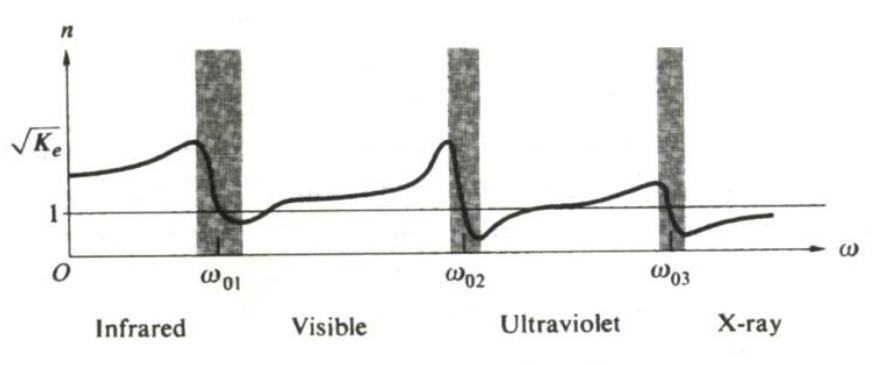
\includegraphics[width=0.7\textwidth]{色散.png}
\end{figure}
光的频率越接近介质的本征频率,介质分子的反应就越剧烈。
\end{enumerate}

\section{Chapter 3}
\begin{enumerate}
\item Scattering:the absorption and prompt re-emission of EM-radiation by electrons associated with atoms and molecules. 投射折射反射本质是都是散射
\item Rayleigh Scattering:要点:1. 粒子比波长小很多 2. 弹性散射 3. 散射强度四次方反比于波长
\begin{equation}
I \propto \frac{1}{\lambda^{4}}
\end{equation}
\item 惠更斯 费马 光程最短原理 (大物知识)\\
光程公式
\begin{equation}
\int n \text{d} s
\end{equation}
\item 用Maxwell推到折射反射定理(超重点)
\begin{enumerate}
\item 设出三个电场(如图)
\begin{figure}
\center
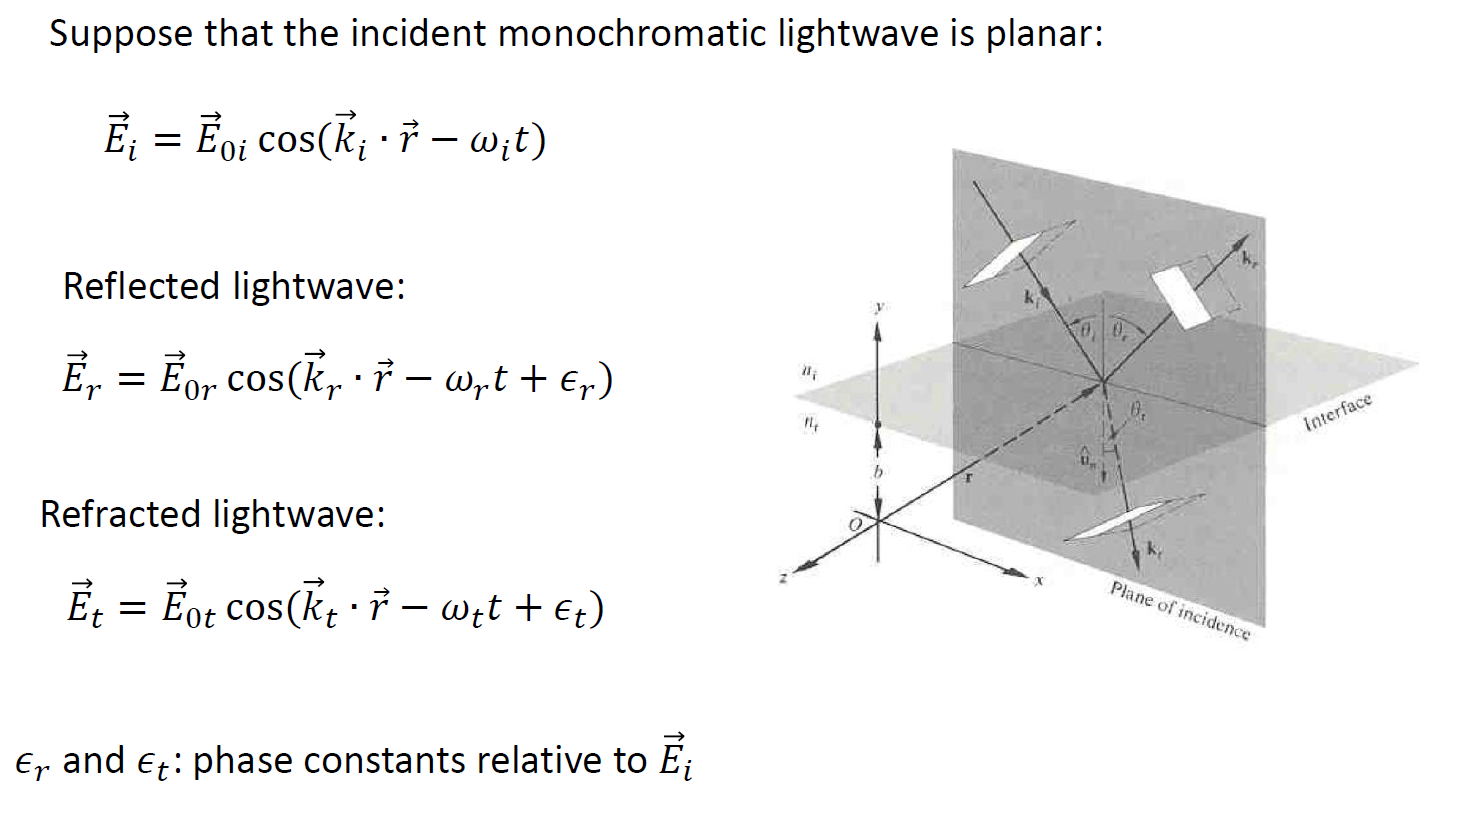
\includegraphics[width=0.7\textwidth]{界面电场.png}
\end{figure}
\item 带入电场边界条件(无散度)(无旋度)
\begin{equation}
\begin{array}{rl}{\hat{u}_{n} \times \vec{E}_{0 i}} & {\cos \left(\vec{k}_{i} \cdot \vec{r}-\omega_{i} t\right)+\hat{u}_{n}} \\ {} & {\times \vec{E}_{0 r} \cos \left(\vec{k}_{r} \cdot \vec{r}-\omega_{r} t+\epsilon_{r}\right)} \\ {} & {=\hat{u}_{n} \times \vec{E}_{0 t} \cos \left(\vec{k}_{t} \cdot \vec{r}-\omega_{t} t+\epsilon_{t}\right)}\end{array}
\end{equation}
上式在任何t都成立,故有
\begin{equation}
\left.\left(\vec{k}_{i} \cdot \vec{r}-\omega_{i} t\right)\right|_{y=b}=\left.\left(\vec{k}_{r} \cdot \vec{r}-\omega_{r} t+\epsilon_{r}\right)\right|_{y=b}=\left.\left(\vec{k}_{t} \cdot \vec{r}-\omega_{t} t+\epsilon_{t}\right)\right|_{y=b}
\end{equation}
又这三个电场的频率应该是一样的,上式变为
\begin{equation}
\left.\left(\vec{k}_{i} \cdot \vec{r}\right)\right|_{y=b}=\left.\left(\vec{k}_{r} \cdot \vec{r}+\epsilon_{r}\right)\right|_{y=b}=\left.\left(\vec{k}_{t} \cdot \vec{r}+\epsilon_{t}\right)\right|_{y=b}
\end{equation}
\item 反射:又上式第一个等号可知
\begin{equation}
\left[\left(\vec{k}_{i}-\vec{k}_{r}\right) \cdot \vec{r}\right]_{y=b}=\epsilon_{r}
\end{equation}
此式在全反射界面是常数。y是垂直于平面的坐标,上式的取值于$r$的平行于界面的分量无关。故$\vec{k}_{i}-\vec{k}_{r}$垂直于反射面,从而有入射角等于反射角。
\item 折射:于反射的情况同理,有
\begin{equation}
\left.\left(\vec{k}_{i} \cdot \vec{r}\right)\right|_{y=b}=\left.\left(\vec{k}_{t} \cdot \vec{r}+\epsilon_{t}\right)\right|_{y=b}
\end{equation}
\begin{equation}
k_{i} \sin \theta_{i}=k_{t} \sin \theta_{t}
\end{equation}
不同之处在于,这两个电场所在的介质不同,所以$|\vec{k}_{i}|\neq |\vec{k}_{t}|$(频率相同,波速不同,波矢长度必然不同)。有关系
\begin{equation}
|\vec{k}_{i}|\frac{c}{n_i}=|\vec{k}_{t}|\frac{c}{n_t}
\end{equation}
\begin{equation}
n_{i} \sin \theta_{i}=n_{t} \sin \theta_{t}
\end{equation}
\end{enumerate}
\item Fresnel Equation (对于偏振光,入射、反射率跟入射角度的关系)
\begin{enumerate}
\item 电场垂直于入射面时(plane-of-incidence,此面垂直于界面) (建议手推一遍保平安):\\
\begin{figure}
\center
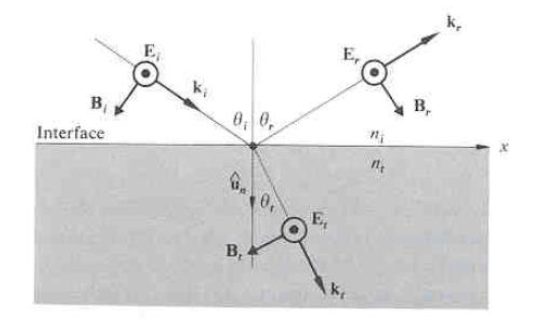
\includegraphics[width=0.7\textwidth]{Fresnel平行.png}
\caption{Fresnel 电场垂直于入射面时}
\end{figure}
推导首先需要磁场的边界条件:
\begin{equation}
H_{\| A}=H_{\| B}
\end{equation}
由此可得
\begin{equation}
-\frac{B_{i}}{\mu_{i}} \cos \theta_{i}+\frac{B_{r}}{\mu_{i}} \cos \theta_{r}=-\frac{B_{t}}{\mu_{t}} \cos \theta_{t}
\end{equation}
又有电场的边界条件
\begin{equation}
E_{0 i}+E_{0 r}=E_{0 t}
\end{equation}
结合两式,注意到电场与磁场的关系是
\begin{equation}
E=\frac{B}{c}=\frac{n B}{c_0}
\end{equation}
我们可以得到
\begin{equation}
r_{\perp} \equiv\left(\frac{E_{0 r}}{E_{0 i}}\right)_{\perp}=\frac{n_{i} \cos \theta_{i}-n_{t} \cos \theta_{t}}{n_{i} \cos \theta_{i}+n_{t} \cos \theta_{t}}
\end{equation}
与
\begin{equation}
t_{\perp} \equiv\left(\frac{E_{0 t}}{E_{0 i}}\right)_{\perp}=\frac{2 n_{i} \cos \theta_{i}}{n_{i} \cos \theta_{i}+n_{t} \cos \theta_{t}}
\end{equation}
\item 电场平行于入射面时:\\
使用与平行时类似的边界条件
\begin{equation}
E_{0 i} \cos \theta_{i}-E_{0 r} \cos \theta_{r}=E_{0 t} \cos \theta_{t}
\end{equation}
\begin{equation}
\frac{B_{i}}{\mu_{i}}+\frac{B_{r}}{\mu_{i}}=\frac{B_{t}}{\mu_{t}}
\end{equation}
要点:平行和垂直,使用的都是磁场和电场在\textbf{垂直界面}方向的边界条件。上式可以推出各种各样的透射率反射率。我觉得背一下定义,推一遍就好。注意 1. 各个比例没有平方,2. 垂直于平行是对入射面说的 3.$r_{\perp},t_{\perp}$的公式对两种情况都一样。正如我们在作业题中做的,这些公式可以用Snell定律化简。
\begin{figure}
\center
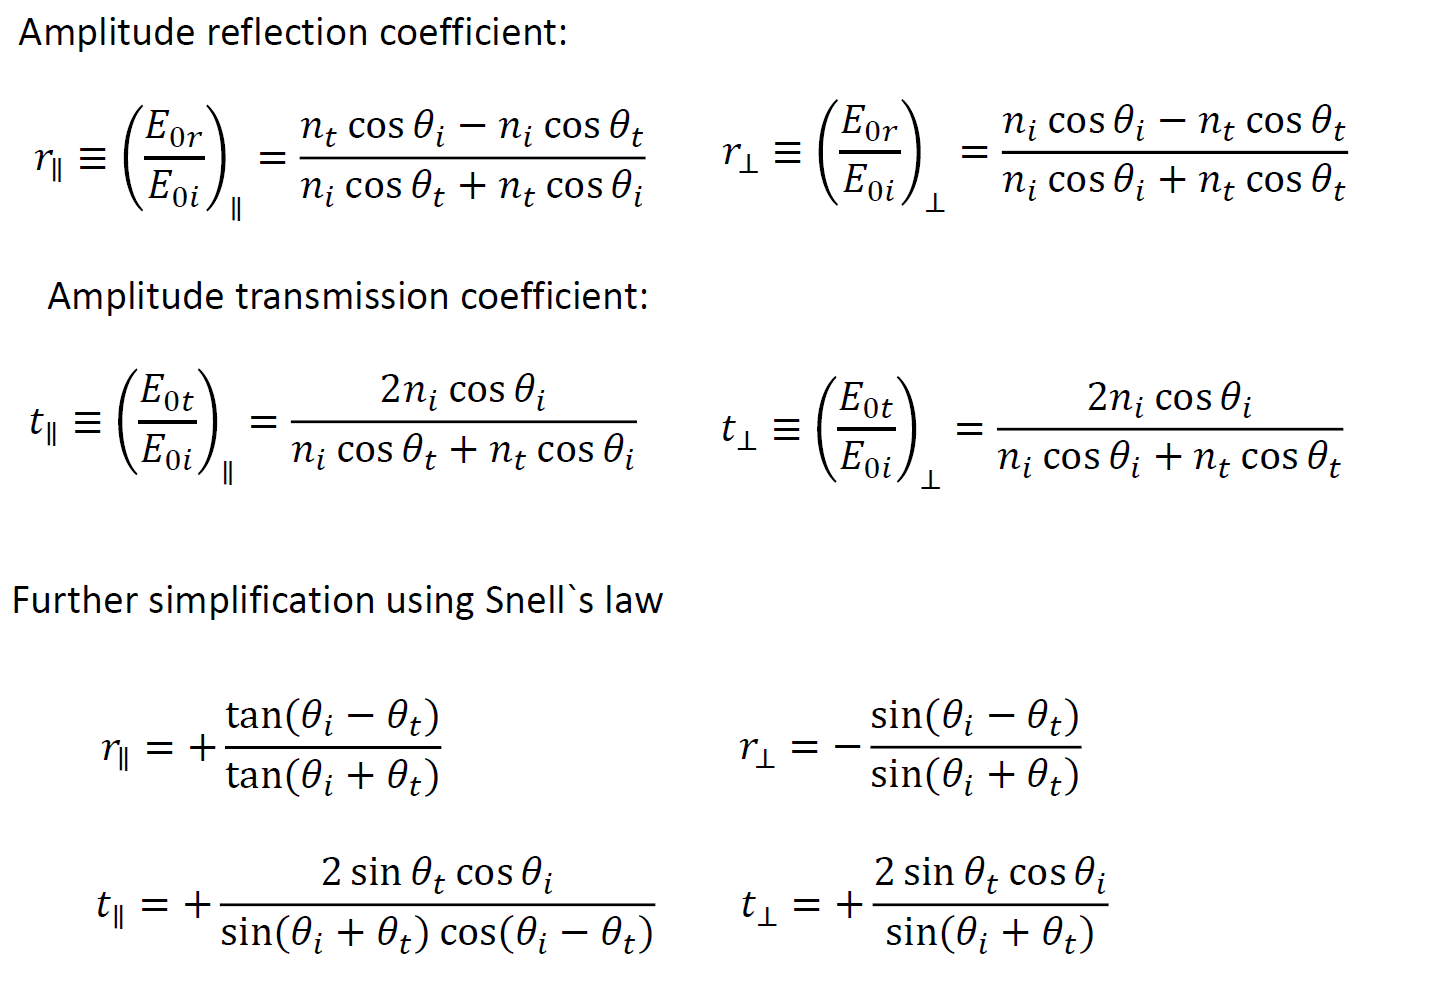
\includegraphics[width=0.7\textwidth]{Fresnel垂直公式表.png}
\caption{Fresnel Equation}
\end{figure}
\end{enumerate}
\item Fresnel Equation 的意义
对于垂直界面打下去的光,有
\begin{equation}
\left[r_{\|}\right]_{\theta_{i}=0}=-\left[r_{\perp}\right]_{\theta_{i}=0}=\left[\frac{n_{t}-n_{i}}{n_{i}+n_{t}}\right]_{\theta_{i}=0}
\end{equation}
\begin{equation}
\left[t_{\|}\right]_{\theta_{i}=0}=\left[t_{\perp}\right]_{\theta_{i}=0}=\left[\frac{2 n_{i}}{n_{i}+n_{t}}\right]_{\theta_{i}=0}
\end{equation}
当入射角和折射角之和为90°时有 ($r_{\|}$)
\begin{equation}
r_{\|}=+\frac{\tan \left(\theta_{i}-\theta_{t}\right)}{\tan \left(\theta_{i}+\theta_{t}\right)}=0
\end{equation}
此时的入射角被称为Polarization angle($\theta_p$)。如果以上的各个比例是负的,说明相位跳了一个$\pi$。就比如当入射角$\theta_i>\theta_p$时,$r_{\|}<0$,反射光水平分量跳$\pi$。对于垂直分量\begin{equation}
r_{\perp}=-\frac{\sin \left(\theta_{i}-\theta_{t}\right)}{\sin \left(\theta_{i}+\theta_{t}\right)}<0
\end{equation}
所以一直跳$\pi$。对于全反射,会有于入射角有关的phase shift。我猜不用掌握其来由。
\item Reflectance and transmittance 
光功率(单位截面,单位时间)
\begin{equation}
I=\langle S \rangle_{T}=\frac{c \epsilon_{0} E_{0}^{2}}{2}
\end{equation}
\begin{figure}
\center
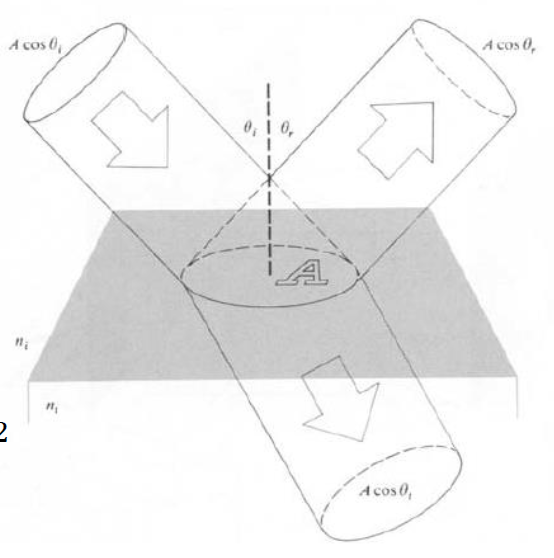
\includegraphics[width=0.5\textwidth]{透反射率.png}
\caption{透反射率}
\end{figure}
根据光功率的定义,其电场的强度大小与密集程度有关,即
对反射($\theta_{i}=\theta_{r}$)
\begin{equation}
R \equiv \frac{I_{r} A \cos \theta_{r}}{I_{i} A \cos \theta_{i}}=\frac{I_{r}}{I_{i}}=\left(\frac{E_{o r}}{E_{0 i}}\right)^{2}=r^{2}
\end{equation}
对投射
\begin{equation}
T \equiv \frac{I_{t} A \cos \theta_{t}}{I_{i} A \cos \theta_{i}}=\frac{n_{t} \cos \theta_{t}}{n_{i} \cos \theta_{i}}\left(\frac{E_{o t}}{E_{0 i}}\right)^{2}=\left(\frac{n_{t} \cos \theta_{t}}{n_{i} \cos \theta_{i}}\right) t^{2}
\end{equation}
故$T\neq t^2$。这点需要注意。
\item 衰逝波 一种指数衰减的波\\
根据 $r_{\|},r_{\perp}$ 的公式可知,当入射角$\theta_i$大于$\theta_c$时,$r$变成虚数,且$r_{\|}r_{\|}^*=r_{\perp}r_{\perp}*=R=1$,$T=0$. 衰逝波是指数衰减因为它不能携带能量。推导的话,用Snell定律算波矢,得到的结果带有虚数,直接带入原方程即可。具体来说
\begin{equation}
\boldsymbol{E}_{t}=\boldsymbol{E}_{0t} \exp i\left(\boldsymbol{k}_{t} \cdot \boldsymbol{r}-\boldsymbol{\omega} t\right)
\end{equation}
其中 (y为垂直于界面的方向)
\begin{equation}
k_{t} \cdot r=k_{t x} x+k_{t y} y
\end{equation}
根据Snell定律 $\cos \theta_{\mathrm{t}}=\left(1-\frac{\sin ^{2} \theta_{\mathrm{i}}}{n_{\mathrm{ti}}^{2}}\right)^{1 / 2}$ (这步是关键,虚数就是这里搞出来的)
\begin{equation}
k_{t y}=k_{\mathrm{t}} \cos \theta_{\mathrm{t}}=\pm k_{\mathrm{t}}\left(1-\frac{\sin ^{2} \theta_{\mathrm{i}}}{n_{\mathrm{ti}}^{2}}\right)^{1 / 2}=\pm i k_{t}\left(\frac{\sin ^{2} \theta_{i}}{n_{t i}^{2}}-1\right)^{1 / 2} \equiv \pm i \beta
\end{equation}
\begin{equation}
k_{t x}=\frac{k_{t}}{n_{t i}} \sin \theta_{i}
\end{equation}
最终
\begin{equation}
\boldsymbol{E}_{t}=\boldsymbol{E}_{0 t} e^{\mp \beta y} e^{i\left(k_{t} x \sin \theta_{i} / n_{t i}-\omega t\right)}
\end{equation}
利用衰逝波可以搞Frustrated total internal reflection(FTIR)。做指纹识别什么的。看课件吧。

\item 金属的光学性质
金属会有电导率$\sigma$,使得Maxwell方程组里的$\vec{J}=\sigma \vec{E}$。 在金属中$\rho=0$。解这样的Maxwell方程组可得
\begin{equation}
\frac{\partial^{2} \vec{E}}{\partial x^{2}}+\frac{\partial^{2} \vec{E}}{\partial y^{2}}+\frac{\partial^{2} \vec{E}}{\partial z^{2}}=\mu \sigma \frac{\partial \vec{E}}{\partial t}+\mu \epsilon \frac{\partial^{2} \vec{E}}{\partial t^{2}}
\end{equation}
非齐次项的存在会使得金属中的电场指数衰减。有 (我猜具体的表达式不会要求推导,电动都没让推,只要记住与光的频率有关就好)
\begin{equation}
\vec{E}=\vec{E}_{0} e^{i(\tilde{k} z-\omega t)} \quad \tilde{k}=k+i \kappa
\end{equation}
有概念skin depth定义为
\begin{equation}
d=\frac{1}{\kappa}
\end{equation}
能量的衰减为
\begin{equation}
I=I_{0} e^{-\alpha z},\alpha=2\kappa
\end{equation}
金属的反射率一般很高。

\end{enumerate}
\section{Chapter 4}
戴老师:第四章重点是\textbf{作业题},不考推导。啊,包括这个得考是吧,Confocal,还有一个什么来着,无限远,这两个必考。要解释到TA能看懂。光阑系统会出问答题。这里面主要考一些概念,比如大光圈会营造一种什么效果啊。什么叫渐晕啊,什么叫景深啊,都要理解。光纤放大器这玩意肯定考,所以顺带着前面光纤你都看。还有可能考密集波分复用。我出题的逻辑是,会把一块内容都包括。先让你算算光纤,后面再让你解答解答这两个技术。所以光纤这部分也是重点。\\

个人评论:这章多说无益,大家去看作业题吧。
\begin{enumerate}
\item Asperical Surface 我没看懂 等时原理?(我猜不考)
\item 薄透镜 Thin-lens equation
\begin{equation}
\frac{1}{s_{o}}+\frac{1}{s_{i}}=\left(n_{l}-1\right)\left(\frac{1}{R_{1}}-\frac{1}{R_{2}}\right)
\end{equation}
从而有焦距公式
\begin{equation}
\frac{1}{f}=\left(n_{l}-1\right)\left(\frac{1}{R_{1}}-\frac{1}{R_{2}}\right)
\end{equation}
\item 光心 Optical Center:光线穿过不会产生偏折的点。作图时很重要。作图就是从像的断点画一根平行的,一条过光心的线。看这两条线在透镜的作用下的交点。(如图)
\begin{figure}
\center
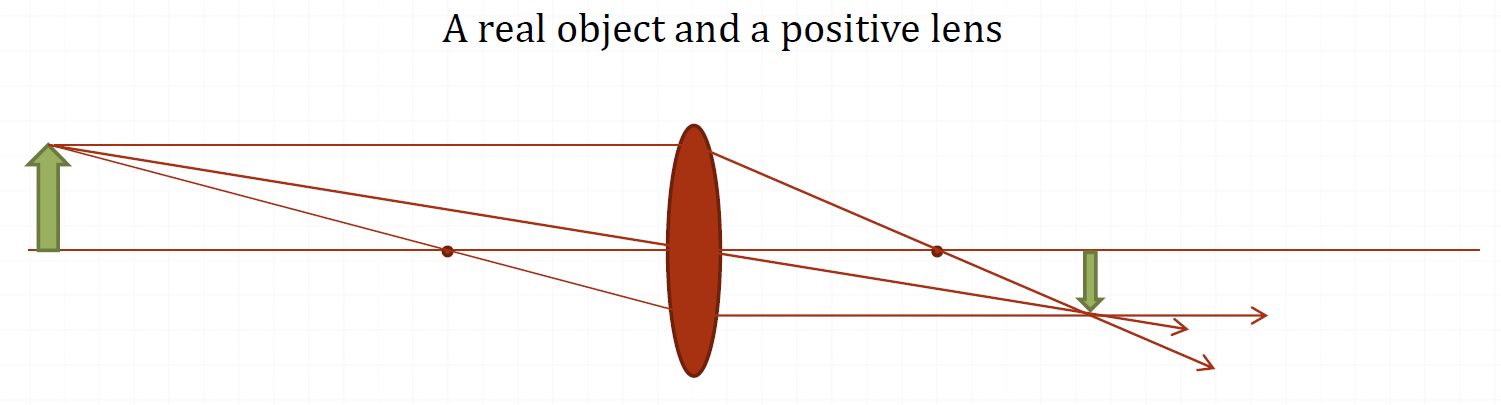
\includegraphics[width=0.7\textwidth]{几何光学作图.png}
\caption{几何光学作图}
\end{figure}
\item 牛顿的透镜成像公式
\begin{equation}
x_{o} x_{i}=f^{2}
\end{equation}
$x_{o}$为物相对于$F_o$(物方焦点)靠左多少。$x_i$为像相对于$F_i$靠右多少。(从左往右成像)
\item Transverse magnification (垂轴放大率)
\begin{equation}
M_{T} \equiv \frac{y_{i}}{y_{o}}=-\frac{s_{i}}{s_{o}}
\end{equation}
Longitudinal magnification  (我觉得不用背,只理解定义就好)
\begin{equation}
M_{L} \equiv \frac{d x_{i}}{d x_{o}}=-\frac{f^{2}}{x_{o}^{2}}=-M_{T}^{2}
\end{equation} 
\item Confocal microscopy (必考,但是我不会,谁来帮帮我)(大家可以参考以下材料)
\href{http://www.physics.emory.edu/faculty/weeks//confocal/}{How does a confocal microscope work?} 
\item Aperture stop 孔径光阑:限制光通过量的(透镜,光阑这种在光路上带边的东西)\\
Field stop 光屏的边缘\\
名词解释
\begin{enumerate}
\item 景深,光圈大小的效果:景深(Depth of Field),是指在摄影机镜头或其他成像器前沿能够取得清晰图像的成像所测定的被摄物体前后距离范围。而光圈、镜头、及拍摄物的距离是影响景深的重要因素。光圈越大(光圈值f越小)景深越浅,光圈越小(光圈值f越大)景深越深。(百度百科)
\item 渐晕:渐晕是离轴越远( 越接近最大视场) 的光线经过光学系统的有效孔径阑越小,所以越离轴的光线在离轴的像面上的光强度就越弱,而形成影像由中心轴向离轴晕开。简单来说,就是轴外光束被拦截的现象称为“渐晕”。(百度百科)
\end{enumerate}
\begin{figure}
\center
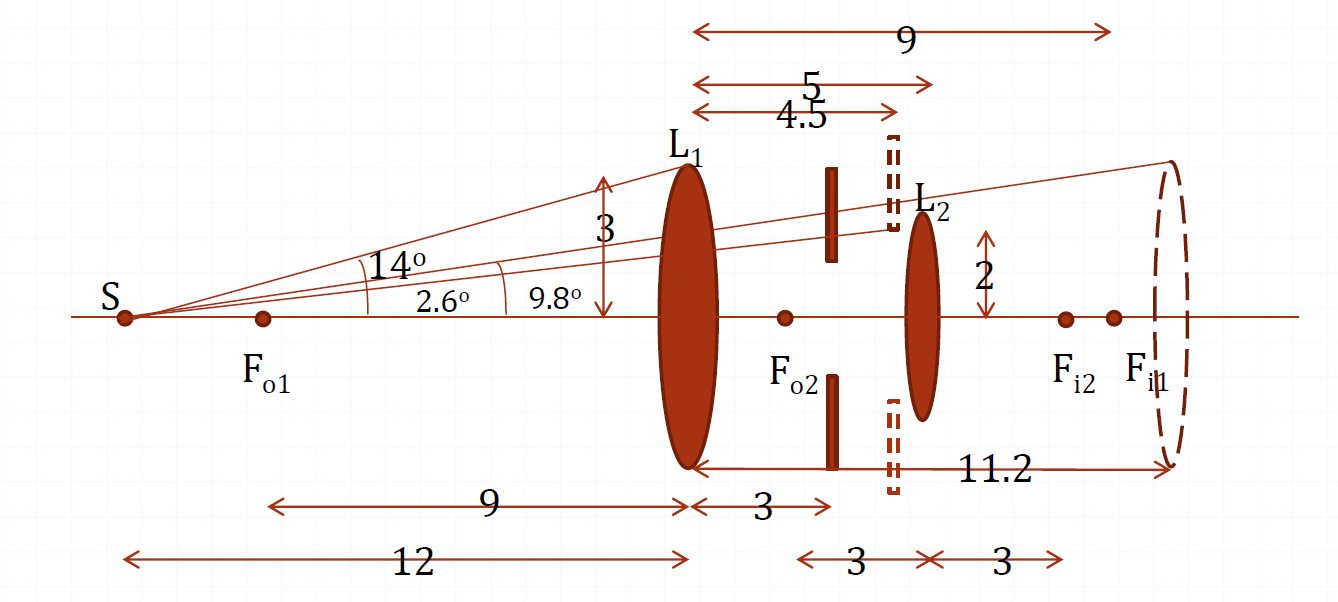
\includegraphics[width=0.7\textwidth]{Pupil.png}
\caption{Pupil神题,做完就行了}
\end{figure}
\item 光纤:
\begin{enumerate}
\item 几何光学:作业题即可。 我想象不到别的考法了。 注意光从空气灌入光纤需要算一次折射就好 (Numerical aperture就一个定义的事($n \sin\theta_{\max}$),我猜可以在考场上问老师,如果忘了的话 )
\item 光纤分类:Stepped-index fiber(cladding(保护层)与core的折射率剧变,第一代技术使用), Graded-index fiber(折射率渐变,intermodal dispersion小). Multimode, Single-mode(大家实验课做过).
\item Intermodal dispersion: 用经典图像处理即可。光速都一样,最短的路径就是直着走,最长的路径就是每次都以critical angle全反射。公式可以现推。
\begin{equation}
\Delta t=t_{\max}-t_{\min}=\frac{L n_{f}}{c}\left(\frac{n_{f}}{n_{c}}-1\right)
\end{equation}
\item Erbium-doped fiber amplifiers:一段掺杂了铒的光纤,Pump light和原信号一起打进去就可以实现信号的放大。
\item Dense wave-length division multiplexing(密集波分复用):不同波长的光承载不同的信号一起灌进光纤,等读取的时候,分离各频率分别读取信号。
\end{enumerate} 
\item 近视:无法聚焦平行光。远视:不能聚焦太近的点发出的光。
\item 无限远光学系统(Infinity optical system)重点在于,这种成像过程中会有一段平行光的部分。在那一部分人们可以加入偏振片,棱镜等保持光的平行的光学元件。
\begin{figure}
\center
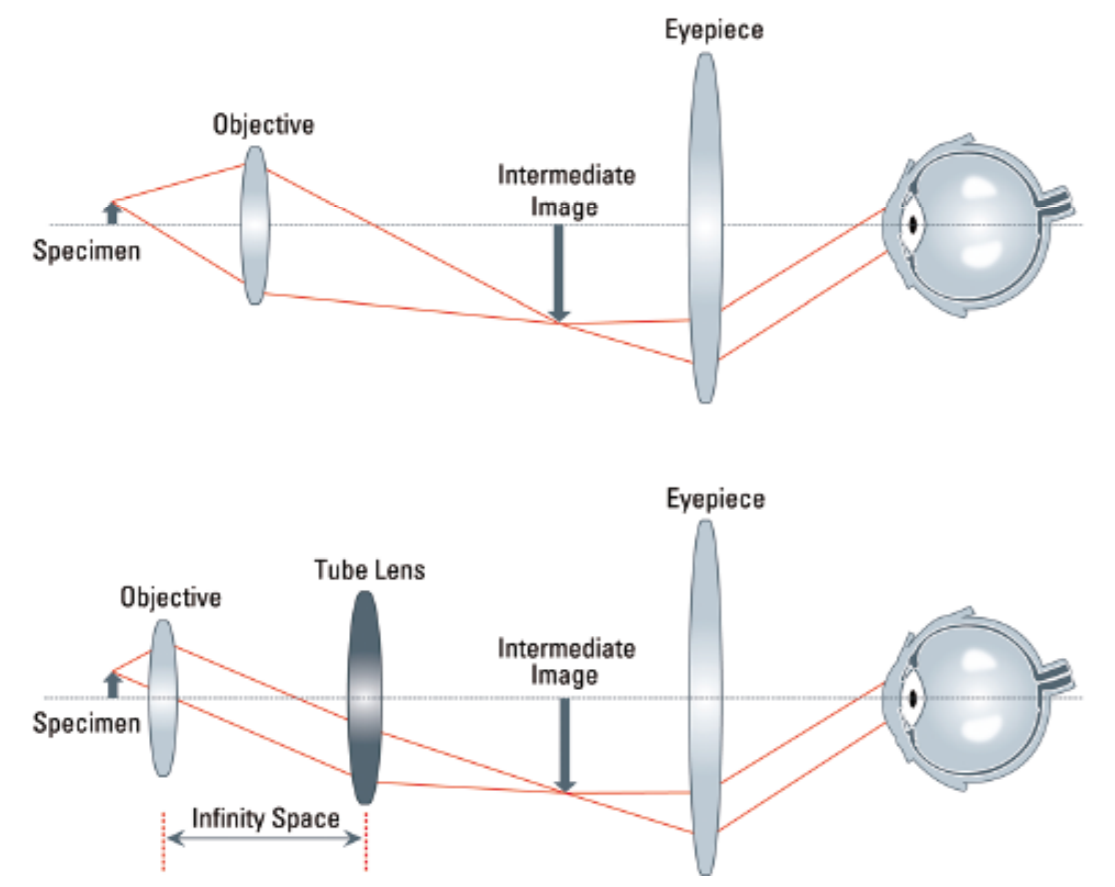
\includegraphics[width=0.5\textwidth]{无限光学系统.png}
\caption{无限远光学系统}
\end{figure}
\end{enumerate}

\section{Chapter 5}
戴老师:矩阵怎么写。矩阵的推导过程,怎么算这个focus。Monochromatic aberration只考球面像差色差,剩下的随便看看。说完了,这也没什么内容。
\begin{enumerate}
\item Ray vector的定义($y$是高度,$\alpha$是角度,$n$是折射率):
\begin{figure}
\center
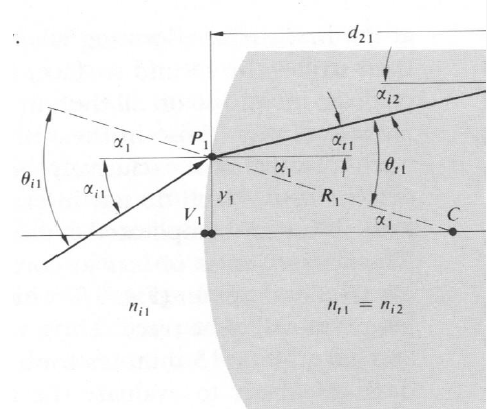
\includegraphics[width=0.5\textwidth]{RayVec.png}
\caption{Ray vector的定义}
\end{figure}
\begin{equation}
\vec{n} \equiv\left[\begin{array}{c}{n \alpha} \\ {y}\end{array}\right]
\end{equation}
习惯上,下标i指入射光,t指出射光。在界面上,Ray vector会经历一个线性变换($\vec{n_{i1}}\to \vec{n_{t1}}$)。
\begin{equation}
\left[\begin{array}{c}{n_{t 1} \alpha_{t 1}} \\ {y_{t 1}}\end{array}\right]=\left[\begin{array}{cc}{1} & {-\mathcal{D}_{1}} \\ {0} & {1}\end{array}\right]\left[\begin{array}{c}{n_{i 1} \alpha_{i 1}} \\ {y_{i 1}}\end{array}\right]
\end{equation}
记为
\begin{equation}
\vec{n_{t1}}=R_1 \vec{n_{i1}}
\end{equation}
在透镜里面,因为透镜有厚度,在到达另一个界面的时候光线的高度会发生变化,有($\vec{n_{t1}}\to \vec{n_{i2}}$)
\begin{equation}
\left[\begin{array}{c}{n_{i 2} \alpha_{i 2}} \\ {y_{i 2}}\end{array}\right]=\left[\begin{array}{cc}{1} & {0} \\ {d_{21} / n_{t 1}} & {1}\end{array}\right]\left[\begin{array}{c}{n_{t 1} \alpha_{t 1}} \\ {y_{t 1}}\end{array}\right]
\end{equation}
\begin{equation}
\vec{n_{i2}}=T_{21}R_1 \vec{n_{i1}}
\end{equation}
最终
\begin{equation}
\vec{n_{t2}}=R_{2}T_{21}R_1 \vec{n_{i1}}
\end{equation}
\item Effective focal length:$\alpha_{i1}$或$\alpha_{t2}$为零时,算出的光线汇聚的位置(如图)。
\begin{equation}
f_{2}=\overline{H_{2} F_{i}}=\frac{y_{i 1}}{-\alpha_{t 2}}
\end{equation}
关于Principal Point我觉得这可以当一个公式背过,因为按照原来的定义想到这个公式比较复杂
\begin{equation}
\overline{H_{2} V_{2}}=\frac{y_{i 1}-y_{t 2}}{-\alpha_{t 2}}
\end{equation}
我不懂的地方:$\alpha$的正负怎么定的。$D_1$怎么算的。
\begin{figure}
\center
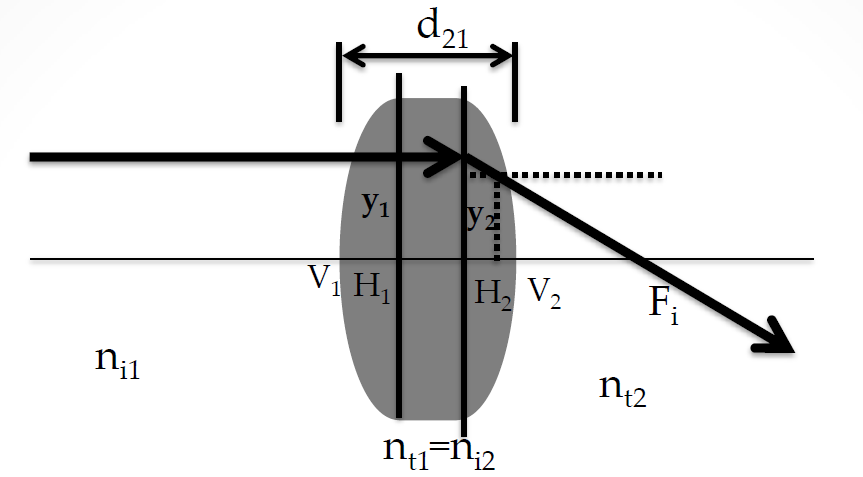
\includegraphics[width=0.5\textwidth]{EffectiveFocal.png}
\caption{Effective focal与Principal Point}
\end{figure}
\item Aberration:只考球面像差色差
\begin{enumerate}
\item 球差:毕竟我们之前做了小角近似。修正方法:1.加光阑使得成像继续满足小角近似。2.如果一面平一面圆,让圆的一面迎光。
\item 色差:因为折射率跟光的频率有关,所以焦距也跟光的频率有关。
\end{enumerate}
\end{enumerate}


\end{document}
